\documentclass[journal,12pt,twocolumn]{IEEEtran}
\usepackage{setspace}
\usepackage{gensymb}
\usepackage{xcolor}
\usepackage{caption}
\usepackage[hyphens,spaces,obeyspaces]{url}


\usepackage{graphicx}
\usepackage{tabularx}

\title{BOOLEAN LOGIC}
\author{prasad deva }

\begin{document}

\maketitle

\section{INTRODUCTION}
\subsubsection{problem}
The boolean logic realized by the logic circuit is
\begin{figure}[h]
    \centering
    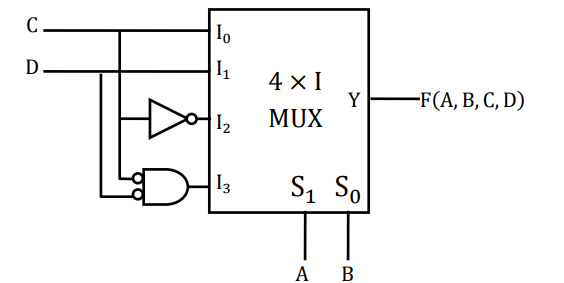
\includegraphics[scale=0.5]{img1.png}
    
    \caption{}

\end{figure}
\section{components}
\subsection{aurdino}
\subsection{bread board}
\subsection{jumper wires - 10}
\subsection{7 segment display}
\subsection{resisitor}
\subsection{7447 IC}
\bigskip
\section{solution}
The equations to be solved by using the boolean logic 
\bigskip

A) $F =\sum(0,1,3,5,9,10,14)$
\bigskip
 
using boolean logic expression the equation expressed as
\bigskip

F = ABD + ACD + BCD + ACD 
\bigskip

B) $F = \sum(2,3,5,7,8,12,13)$
\bigskip

using boolean expression the equation expressed as 
\bigskip

F =ABC + ABD + ABC + ACD   
\bigskip

using boolean expression the equation expressed as
\bigskip

C) $F = \sum(1,2,4,5,11,14,15)$
\bigskip

using boolean expression the equation expressed as
\bigskip

F = ABC + ACD + ABC + ACD 
\bigskip

D) $F = \sum(2,3,5,7,8,9,12)$
\bigskip

using boolean expression the equation expressed as
\bigskip

F = ABC + ABD + ABC + ABCD 
\bigskip

\begin{table}[h]
    \setlength{\arrayrulewidth}{0.5mm}
\setlength{\tabcolsep}{18pt}
    \centering
\begin{tabular}{|c|c|c|c|c|}
  \hline
    \textbf A &\textbf B &\textbf C & \textbf D &\textbf F  \\
       \hline
     0&0&0&0&0 \\
     0&1&0&0&0 \\
     1&0&0&0&1 \\
     1&1&0&0&1 \\
     0&0&0&1&0 \\
     0&0&1&0&0 \\
     0&0&1&1&1 \\
     0&1&0&1&1 \\
     0&1&1&0&0 \\
     0&1&1&1&1 \\
     1&0&0&1&0 \\
     1&0&1&0&1 \\
     1&0&1&1&1 \\
     1&1&0&1&1 \\
     1&1&1&0&1 \\
     1&1&1&1&1 \\
       \hline
\end{tabular}
\caption{Truth Table}
\end{table}
\bigskip

\bigskip
 solution of the logic circuit is
\bigskip

$F = \sum(2,3,5,7,8,9,12)$
\bigskip

F = ABC+ ABD + ABC+ ABCD
\end{document}
 
